\section{System Design and Architecture}\label{sec:system}

\subsection{Overall Architecture}
The proposed system is a multi-layered pipeline that transforms raw blockchain data into a searchable semantic index. The architecture, shown in Fig.~\ref{fig:architecture}, consists of five primary layers: Data Access, Data Extraction, Data Modeling \& Storage, Semantic Enrichment, and Search \& Retrieval. Fig.~\ref{fig:process} shows the components and the process inside the system.

\begin{figure}[htbp]
	\centerline{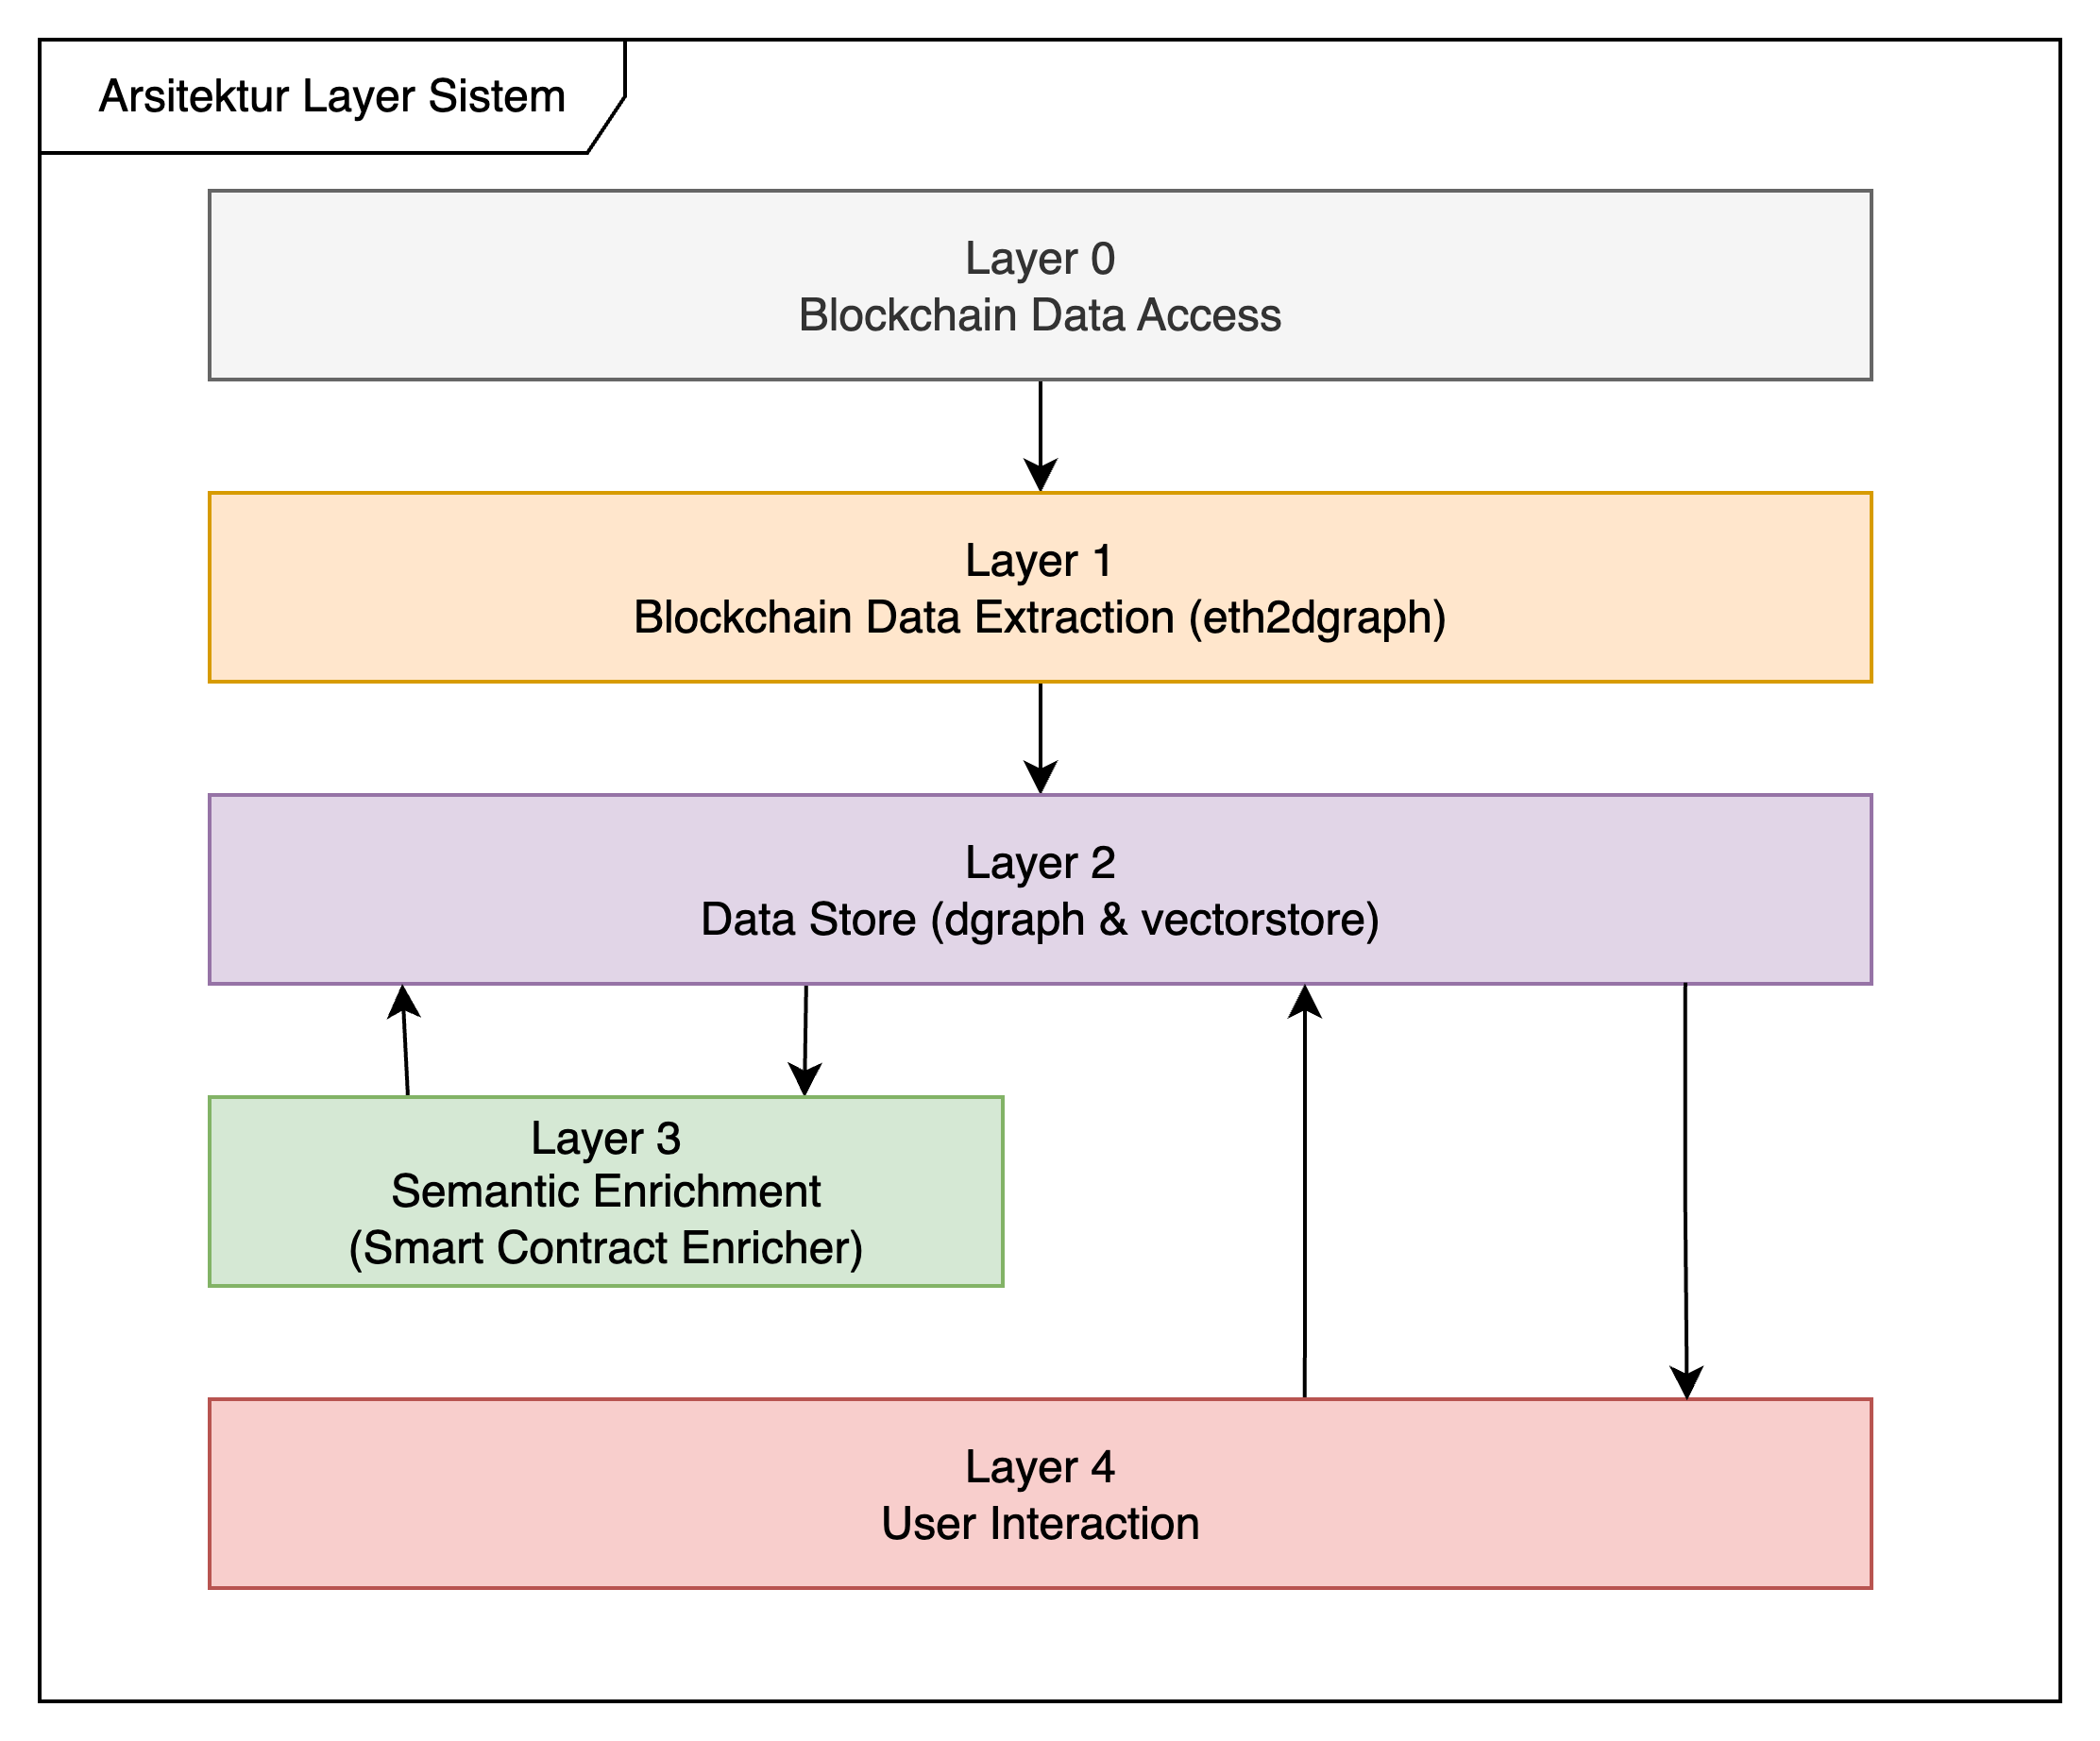
\includegraphics[width=0.48\textwidth]{resources/chapter-3/layer-arsitektur-new.png}}
	\caption{High-level system architecture.}\label{fig:architecture}
\end{figure}

\begin{figure}[htbp]
	\centerline{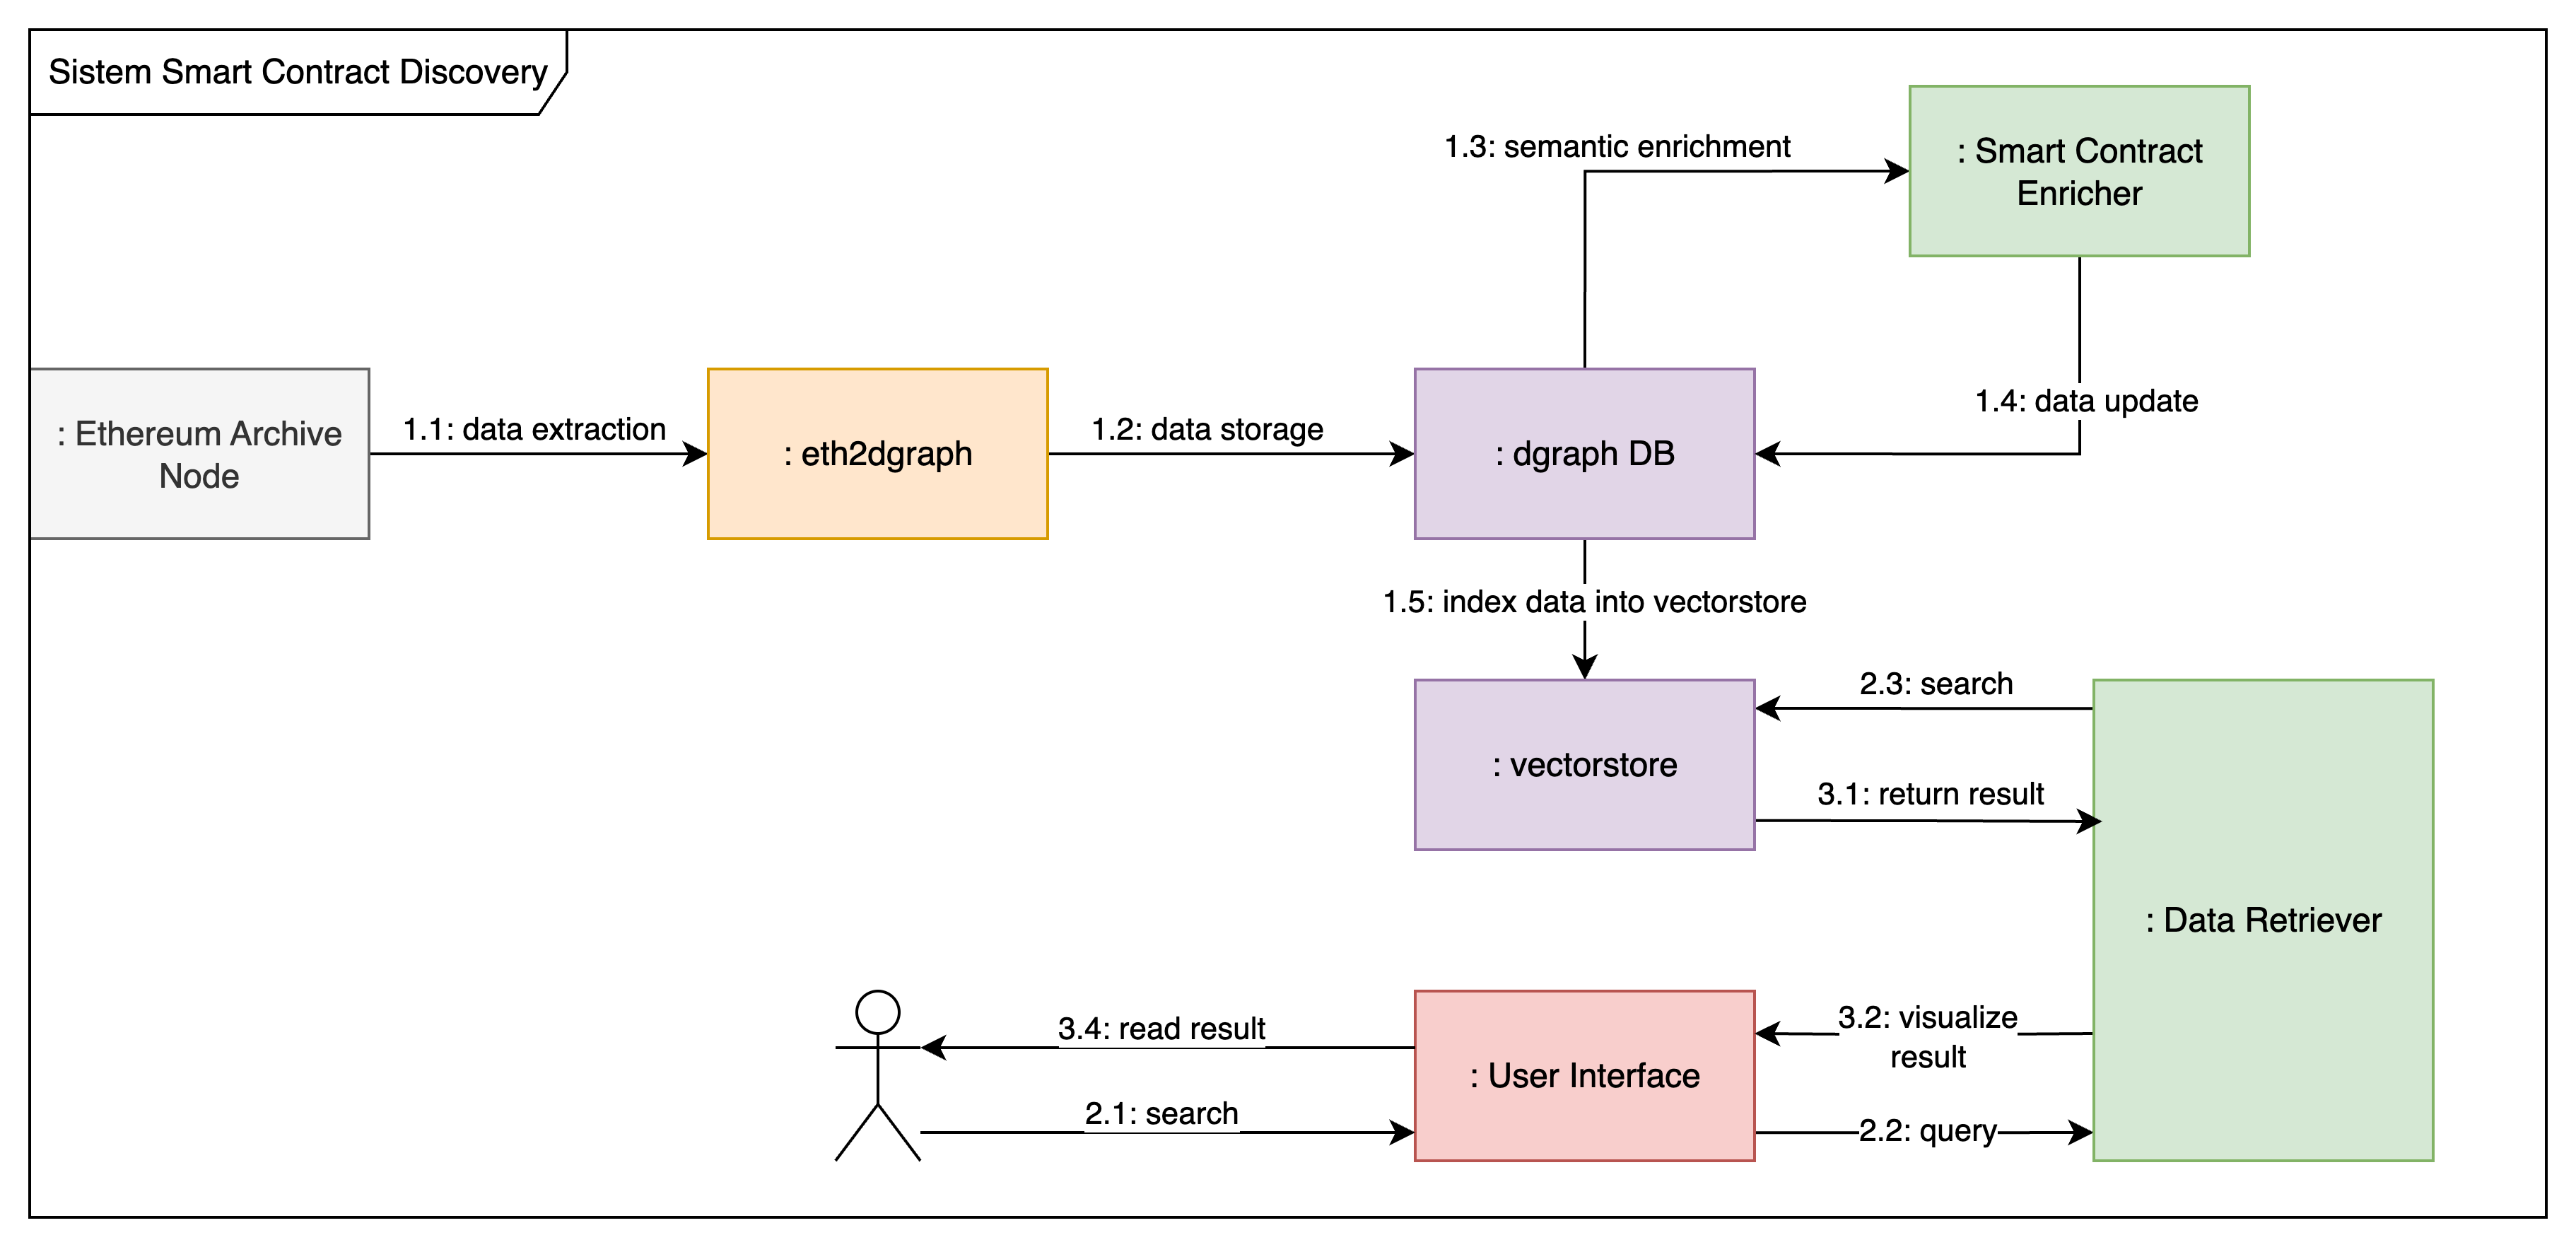
\includegraphics[width=0.48\textwidth]{resources/chapter-3/komponen-utama-new.png}}
	\caption{High-level system process.}\label{fig:process}
\end{figure}

\subsection{Data Extraction and Modeling}
The process begins with extracting data from an Ethereum Archive Node. We use the eth2dgraph tool~\cite{b7} for this task, as it efficiently extracts contract deployments and links them to verified source code from repositories like Smart Contract Sanctuary~\cite{b10}. The extracted data is loaded into Dgraph, a distributed graph database. Then, a schema that holds placeholders for semantic enrichment results are applied to the data.

\subsection{The Semantic Enrichment Pipeline}
This pipeline is the core of our contribution. For each contract with verified source code, we perform semantic enrichment using an LLM (OpenAI's GPT-4o mini). The process is as follows:
\begin{enumerate}
	\item \textbf{Input Preparation:} The flattened Solidity source code of a contract is fed into the LLM.
	\item \textbf{Prompt Engineering:} A carefully designed prompt instructs the LLM to act as an expert smart contract auditor and return a single, minified JSON object based on a strict schema.
	\item \textbf{Structured JSON Generation:} The LLM analyzes the code and generates a JSON object containing key fields such as:
	      \begin{itemize}
		      \item \texttt{description}: A high-level summary of the contract's purpose.
		      \item \texttt{standards}: A list of implemented ERC/EIP standards (e.g., erc-20, eip-1967).
		      \item \texttt{patterns}: A list of common design patterns (e.g., proxy\_uups, access\_control\_ownable).
		      \item \texttt{functionalities}: Granular tags for specific actions (e.g., token\_minting, onchain\_voting).
		      \item \texttt{application\_domain}: The single most evident domain (e.g., defi\_dex, nft\_collection).
		      \item \texttt{security\_risks\_description}: \\A brief analysis of potential security risks.
	      \end{itemize}
\end{enumerate}

This structured output is then saved back into the corresponding ContractDeployment node in Dgraph. The LLM used in the pipeline leverages LangChain's adaptor to quickly switch models based on configuration.

\subsection{Semantic Retrieval Mechanism}
To enable fast and accurate search, we use a vector-based retrieval mechanism:

\begin{itemize}
	\item \textbf{Embedding Generation:} The enriched JSON object for each contract is serialized into a descriptive string. This string is then converted into a high-dimensional vector embedding using a sentence-transformer model (BAAI/bge-small-en-v1.5). These embeddings are stored and indexed in Dgraph.
	\item \textbf{Query Processing:} A user's natural language query (e.g., ``upgradable contracts'') is converted into a vector embedding using the same model.
	\item \textbf{Vector Search:} We use Dgraph's built-in HNSW (Hierarchical Navigable Small World) index to find the contract embeddings closest to the query embedding, measured by Cosine Similarity. The system returns a ranked list of the most relevant contracts.
\end{itemize}

\section{Implementation and Evaluation}\label{sec:implementation}

\subsection{Implementation Details}
The system backend was built with Python using the FastAPI framework. Dgraph served as both the graph and vector database. The enrichment process was powered by the OpenAI API, and embeddings were generated using the HuggingFace Transformers library. A web-based UI was developed using Next.js.

\subsection{Experimental Setup}
We conducted an experiment on a dataset of 118 verified smart contracts extracted from the Ethereum mainnet to validate our approach.

\textbf{Metric:} We used Precision@10 as the primary evaluation metric. Relevance was determined by manual evaluation against a pre-defined, objective rubric based on verifiable source code evidence (e.g., inheritance from Ownable.sol, use of DELEGATECALL).

\textbf{Baselines:} We compared our method against two baselines:
\begin{itemize}
	\item Baseline 1 (Keyword-Source): Full-text search on raw source code.
	\item Baseline 2 (Keyword-Semantic): Full-text search on the LLM-generated descriptions.
	\item Proposed Method (Vector Search): Our semantic search using vector embeddings.
\end{itemize}

\textbf{Queries:} A set of 20 queries was used, ranging from simple keywords (``erc-20'') to complex natural language descriptions (``contracts that can be upgraded...'').

\subsection{Results and Analysis}
The results of our evaluation, summarized in Table~\ref{tab:results}, demonstrate the clear superiority of our semantic search approach.

\begin{table}[htbp]
	\caption{Precision@10 Results}\label{tab:results}
	\begin{center}
		\begin{tabular}{l l c}
			\toprule
			\textbf{Search Method}   & \textbf{Query Type} & \textbf{Average Precision} \\
			\midrule
			Keyword-Source           & Keyword             & 39.2\%                     \\
			Keyword-Semantic         & Keyword             & 49.0\%                     \\
			Keyword-Semantic         & Natural Language    & 27.5\%                     \\
			Vector Search (Proposed) & Keyword             & 72.5\%                     \\
			Vector Search (Proposed) & Natural Language    & 65.0\%                     \\
			\bottomrule
		\end{tabular}
	\end{center}
\end{table}

Our proposed vector search method significantly outperformed both baselines, achieving 72.5\% precision with keyword queries and 65.0\% with natural language queries. Keyword search on raw source code was the least effective (39.2\%), highlighting its inability to grasp context.

The analysis reveals that semantic search succeeds because it understands intent. For instance, for the query ``contracts that can be upgraded,'' a keyword search might find contracts containing the word ``upgrade'' but miss those implementing a proxy pattern without using that specific term. Our system, however, identifies the proxy\_uups or proxy\_transparent patterns during enrichment, allowing it to correctly retrieve these contracts. The LLM-generated descriptions serve as a powerful intermediate representation that bridges the semantic gap between a developer's needs and the contract's code.

The system also proved feasible for large-scale application. The average cost for enriching a single contract was approximately \$0.002, with a median processing time of 5.56 seconds. Query latency for vector search was consistently low, with a median of 76 ms.

\section{Conclusion and Future Work}\label{sec:conclusion}

\subsection{Conclusion}
This paper presented a Smart Contract Discovery System that addresses the critical challenge of discovering deployed smart contracts and public on-chain infrastructure. By leveraging Large Language Models to create a deep semantic understanding of source code and making it searchable via natural language, our system provides a highly effective and precise method for finding functionally relevant contracts. The empirical results confirm that this approach can significantly improve developer workflow, promote better integration with existing on-chain infrastructure, and contribute to a more efficient and composable blockchain ecosystem.

\subsection{Future Work}
There are several promising directions for future research. First, the system could be extended to use another conversational AI layer to understand user's intent and craft a requirement query. Second, the retrieval mechanism could be enhanced by implementing a re-ranking stage that combines semantic similarity with on-chain metrics like transaction count or security audit history. Finally, the rich, structured data from our pipeline could be used to construct a comprehensive knowledge graph of the smart contract ecosystem, enabling deeper insights into the relationships and dependencies within the decentralized world.